% This is the Reed College LaTeX thesis template. Most of the work 
% for the document class was done by Sam Noble (SN), as well as this
% template. Later comments etc. by Ben Salzberg (BTS). Additional
% restructuring and APA support by Jess Youngberg (JY).

\documentclass[12pt,twoside]{reedthesis}
\usepackage{graphicx,latexsym} 
\usepackage{amssymb,amsthm,amsmath}
\usepackage{longtable,booktabs,setspace} 
\usepackage[hyphens]{url}
\usepackage{rotating}

\usepackage{xcolor}

% \usepackage{natbib}
% Comment out the natbib line above and uncomment the following two lines to use the new 
% biblatex-chicago style, for Chicago A. Also make some changes at the end where the 
%bibliography is included. 
\usepackage[authordate,autocite=inline,backend=biber, natbib]{biblatex-chicago}
\addbibresource{thesis.bib}

% \usepackage{times} % other fonts are available like times, bookman, charter, palatino

\title{Yay Copepods}
\author{Ella Crotty}
% The month and year that you submit your FINAL draft TO THE LIBRARY (May or December)
\date{May 2025}
\division{Environmental Studies}
\advisor{Sam Fey}
%If you have two advisors for some reason, you can use the following
\altadvisor{Zachary Gold}
%%% Remember to use the correct department!
\department{Biology}
% if you're writing a thesis in an interdisciplinary major,
% uncomment the line below and change the text as appropriate.
% check the Senior Handbook if unsure.
\thedivisionof{The Established Interdisciplinary Committee for}
% if you want the approval page to say "Approved for the Committee",
% uncomment the next line
%\approvedforthe{Committee}

\setlength{\parskip}{0pt}

\begin{document}

  \maketitle
  \frontmatter % this stuff will be roman-numbered
  \pagestyle{empty} % this removes page numbers from the frontmatter

    \chapter*{Acknowledgements}
	I want to thank a few people.
	And test my citations \autocite{Barth2024}.

% The preface is optional
% To remove it, comment it out or delete it.
    \chapter*{Preface}
	This is an example of a thesis setup to use the reed thesis document class.
	
    \chapter*{List of Abbreviations}
		You can always change the way your abbreviations are formatted. Play around with it yourself, use tables, or come to CUS if you'd like to change the way it looks. You can also completely remove this chapter if you have no need for a list of abbreviations. Here is an example of what this could look like:

	\begin{table}[h]
	\centering % You could remove this to move table to the left
	\begin{tabular}{ll}
		\textbf{ENSO}  	&  El Ni\~{n}o Southern Oscillation \\
		\textbf{OCNMS}  	&  Olympic Coast National Marine Sanctuary \\
		\textbf{OMZ}  	&  Oxygen Minimum Zone \\
		\textbf{IPC}  	&  Intergovernmental Policy Council \\
		\textbf{NOAA}  	&  National Oceanic and Atmospheric Administration \\
		\textbf{PMEL}  	&  Pacific Marine Environmental Laboratory \\
		\textbf{OME}  	&  Ocean Molecular Ecology \\
		\textbf{PPS}  	&  Phytoplankton and Particle Sampler \\
		\textbf{DVM}  	&  Daily Vertical Migration \\
	\end{tabular}
	\end{table}
	

    \tableofcontents
    \listoftables
    \listoffigures

% If your abstract is longer than a page, there may be a formatting issue.
    \chapter*{Abstract}
	The preface pretty much says it all.
	
	\chapter*{Dedication}
	You can have a dedication here if you wish.

  \mainmatter % here the regular arabic numbering starts
  \pagestyle{fancyplain} % turns page numbering back on

%The \introduction command is provided as a convenience.
%if you want special chapter formatting, you'll probably want to avoid using it altogether

    \chapter*{Introduction}
         \addcontentsline{toc}{chapter}{Introduction}
	\chaptermark{Introduction}
	\markboth{Introduction}{Introduction}
	% The three lines above are to make sure that the headers are right, that the intro gets included in the table of contents, and that it doesn't get numbered 1 so that chapter one is 1.

% \onehalfspacing
% \doublespacing
	
	

\section{Climate Change, Hypoxia, and OCNMS}

Due to human greenhouse gas emissions, the Earth's oceans are warming and losing oxygen. Over 90\% of the excess heat trapped by greenhouse gases has been absorbed by the ocean, causing a significant increase in temperature in most regions in the ocean \autocite{Bindoff2013}. According to the United Nations Intergovernmental Panel on Climate Change, the global sea surface temperature has risen 0.65 ºC above pre-industrial levels as of 2022 \autocite{Portner2019}. This warming has reduced the solubility of dissolved oxygen in water, which accounts for 15-50\% of the climate change driven oxygen decrease in the global ocean \autocite{Helm2011, Ito2017, Schmidtko2017}. The loss of 0.5-3.3\% of the open ocean's oxygen down to 1000 m depth is very likely, and it is very likely that oxygen minimum zones are expanding \autocite{Bindoff2013}. This decline has been particularly pronounced in the North Pacific, where this study is located \autocite{Bindoff2013, Ito2017}. The rest of the decrease is caused by decreased sea-air and surface ocean-deep ocean oxygen flux due to increasing stratification \autocite{Barth2024, Mancini2024, Portner2019}. Ocean stratification refers to the way that layers of ocean water with different densities form, restricting heat, carbon, and oxygen exchange between layers of different depths. This density difference is primarily caused by differences in temperature and salinity between water masses. As the ocean's surface water warms, it becomes less dense, increasing the magnitude of the density difference between surface and deep waters and increasing stratification by 5.3\% globally between 1960 and 2018 \autocite{Li2020a}. This increased stratification decreases the flow of nutrients and oxygen to the deeper layers of the ocean. 

The surface ocean contains more oxygen than deeper waters, because the atmosphere and the surface ocean rapidly exchange oxygen in order to equilibrate the partial pressure of oxygen in both systems \autocite{Ito2010}. According to a 1948 study, 40\% of air-sea exchange at a study site in the Gulf of Maine was due to organisms producing and consuming oxygen, while the remaining 60\% of the exchange was due to the solubility of oxygen in water \autocite{Redfield1948}. Because the upper ocean receives sunlight, phytoplankton live there and photosynthesize, producing oxygen that primarily remains in the ocean \autocite{Li2020}. However, the rate at which oxygen leaves the ocean is increasing as the ocean's temperature increases \autocite{Li2020}. Ocean circulation moves this oxygen to the deep ocean over the course of centuries, where the oxygen is consumed via respiration but cannot be replenished by photosynthesis or atmospheric exchange \autocite{Karstensen2008, Deutsch2024, Ito2010}. As a result, deeper ocean waters are lower in oxygen, and the middle of the water column is the most oxygen-poor due to its relative stillness, with the Oxygen Minimum Zone (OMZ) in the middle of the Pacific Ocean water column ranging from less than \textcolor{red}{ [1 µmol/kg] to [45 µmol/kg] compared to the  [61-120 µmol/kg]} of shallower waters along the Oregon and Washington coasts in the summertime \autocite{Karstensen2008, Deutsch2024, Barth2024, Pierce2012, Wyrtki1962}. 

As a result of these interactions, as well as increased nutrient inputs from agriculture causing eutrophication, hypoxic events in which the oxygen concentration in water becomes low enough to harm or kill marine organisms are increasing in frequency, duration, and severity throughout the world's oceans. Most marine organisms require oxygen to survive, and these hypoxic events can cause severe fish die-offs or force migrations which change the distribution of species \autocite{Pihl1991, Miller2002}. Because different species have different tolerances to hypoxia and different levels of mobility, not all species distributions will be affected in the same way by hypoxia, which may result in predator and prey populations becoming offset from each other. 

Understanding the effects of this global decrease in ocean oxygen levels is crucial to predicting the overall effects of climate change on the oceans and to developing climate-aware management strategies for marine resources. Studies of the effects of hypoxia on marine organisms use a variety of lab and fieldwork methods. Laboratory experiments on hypoxia's effects typically involve subjecting organisms to different levels of dissolved oxygen over a certain period of time, then measuring factors such as survival, growth rate, metabolism, and reproductive rate in order to determine whether the hypoxia has a negative effect \autocite{Steckbauer2020}. Field studies typically entail measuring dissolved oxygen levels and organismal abundance, using methods such as satellite tagging and trawl surveys that vary by scale and organism type (for example, \autocite{Keister2020}). Field experiments have more ecological relevance, but present difficulties in untangling the effects of other environmental factors \autocite{Borges2022, Boyd2018}. 

This study will focus on hypoxia in Olympic Coast National Marine Sanctuary (OCNMS), off the coast of Washington state, U.S.A.. The Olympic Coast is an upwelling zone, meaning that when summer winds push the surface water offshore, nutrient-rich and oxygen-poor water flows upwards from the deep Pacific Ocean towards the coast \autocite{OceanographyOlympicCoast, Hickey2003}. After this oxygen-poor water reaches the shallower waters of the continental shelf, respiration and decaying organic matter on the continental shelf reduce the water's oxygen content even further \autocite{Pierce2012}. Hypoxic events in OCNMS often occur in the summer, are driven by upwelling, not nutrient runoff, and are increasing in severity \autocite{Barth2024}. Hypoxic zones have occurred annually in the US Pacific Northwest since 2002, and their increasing size and severity has been linked to climate change. These nutrients sustain a rich ecosystem with high primary productivity, but as oceans warm and the deep water gets progressively more hypoxic, the seasonal hypoxic events in OCNMS are increasing in their severity and duration, which will eventually harm organisms more than the nutrients help them. Additionally, as climate change warms the land and ocean at different rates, the summer winds that cause upwelling are getting stronger, resulting in upwelling events that push more deep water up towards the coast \autocite{Barth2024}. 

OCNMS is located off the Olympic Peninsula of Washington state, and extends 25 to 45 miles into the ocean. It regularly experiences rough seas, wave heights up to 49 feet, and intense winter storms. The sanctuary contains a wide variety of habitats, including rocky shores, kelp forests, sandy seafloor, and deep ocean canyons. The sanctuary is home to many marine mammals, fish, invertebrates, and seaweeds, and is a major feeding area for migrating seabirds. The sanctuary covers habitat for rockfish, salmon, halibut, Dungeness crab and other ecologically, commercially, and culturally important species of the Olympic Coast \autocite{FishOlympicCoast}.  Within the sanctuary, prohibited activities include oil, gas, and mineral development; discharging certain types of waste from boats; moving or injuring historical resources; seabed drilling; taking or possessing any marine mammal, bird, or turtle; disturbing marine mammals or birds with low-flying aircraft; Department of Defense bombing activities \autocite{15CFRPart}. The Olympic Coast National Marine Sanctuary Advisory Council provides advice on the sanctuary's management. The council is comprised of representatives of Native American tribes, state and local governments, other federal agencies, maritime industry, fishing, education, tourism, conservation organizations, and the community. The sanctuary lies within the Usual and Accustomed treaty fishing, hunting, and gathering areas of the Hoh Tribe, Makah Tribe, Quileute Tribe, and the Quinault Indian Nation, or the Coastal Treaty Tribes. Fisheries and other marine resources off the Olympic Coast are co-managed by the state of Washington, the United States (specifically the National Oceanographic and Atmospheric Administration's Office of National Marine Sanctuaries), and the Coastal Treaty Tribes, who formed the Olympic Coast Intergovernmental Policy Council (IPC) in 2007 to provide a forum for resource managers \autocite{IntergovernmentalPolicyCouncil}.
	
\section{Environmental DNA}

Environmental DNA (eDNA) is the genetic material present in the environment, including extracellular DNA, fragments of cells and tissues, and entire small organisms \autocite{Power2023}. In marine environments, eDNA can be filtered out of the water and sequenced to detect many species at the place and time where the water sample was collected. eDNA is a powerful tool for detecting multiple species at once with relatively little sampling effort, but it cannot detect more specific data such as size, sex, and age. The general process of eDNA sampling begins by physically filtering seawater with 0.4 micron filters, then extracting and amplifying the resulting DNA and chromosome fragments using polymerase chain reaction (PCR) \autocite{Power2023}. PCR for eDNA studies is conducted using general primers, small pieces of DNA that attach to and duplicate regions of DNA common across species. After this amplification, the resulting fragments of DNA are sequenced using high-throughput sequencing and then identified using a process called metabarcoding. The sequence fragments are compared to a reference database of genes sequenced from known species, allowing the species present in the water column at the time of sampling to be identified through only a small region of their genome known as a barcoding region \autocite{Miya2022}. eDNA can detect species with relatively high spatial resolution, from as little as 60 meters in a kelp forest \autocite{Port2016}| to 800 meters in deep-water habitats in Maizuru Bay, Japan \autocite{Yamamoto2017}, because eDNA levels drop below the detection limit soon after being released via diffusion and decay. However, our understanding of how far eDNA can migrate in the environment is still relatively limited, and eDNA dispersal and decay can be affected by a number of environmental factors \autocite{Cristescu2018}. Because of the high sensitivity of eDNA methods, contamination must be diligently avoided. Because metabarcoding requires reference sequences, any species whose barcoding region in question has not been sequenced cannot be detected by a study \autocite{Miya2022}. This is not an issue with heavily-studied species like salmon, but can present an issue in other areas. eDNA metabarcoding results provide read abundances, or numbers of DNA fragments, but these are affected by PCR replication efficiency, so they are difficult to compare between different species and methods \autocite{Miya2022}. While it is difficult to get quantitative results from eDNA, it is possible to calculate a metric of relative abundance within species known as eDNA index. Kelly et al. used simulations and found that this index accurately captures trends in the biomass of detected organisms. eDNA index is calculated in two steps. First, the read counts of each species within a sample are converted to a proportion of reads within the sample. Then, within each species, those proportions are normalized to range from zero to 1. After this, each species has one sample where it has an eDNA index of one, and that is the sample where that species was most abundant. This method cannot be used to compare different species, only to determine trends within each species, and it will be used in this study \autocite{Kelly2019}.

Since 2021, the National Oceanic and Atmospheric Administration's Pacific Marine Environmental Laboratory (NOAA PMEL) has been collecting eDNA samples in OCNMS using a modified McLane phytoplankton and particulate sampler (PPS).  The PPS was deployed for three, month-long intervals between May 2021 and August 2022, at the Teawhit Head 42 meter depth mooring (\textcolor{red}{see Figure} [OCNMSbuoymap]). This sampler collected, filtered, and preserved 1 L water samples every 36 hours, and the samples were then amplified for 5 metabarcoding markers. Samples were taken using 0.4 micron filters taken off the sampler and preserved in ethanol, and the extracted DNA was amplified using several primers. This study focuses on the species identifications that used the MiFish (12S rRNA primer designed for fish) and CO1 (mitochondrially encoded cytochrome c oxidase I, a common barcoding gene for studies on eukaryotes) primers. Amplified regions were sequenced and matched to available reference genomes, resulting in species detection data that includes the number of reads (DNA strands) of each species detected. 

My summer 2024 research included combining the results of these eDNA detections with oceanographic measurements collected by the Teahwhit Head oceanographic mooring, where the PPS sampler was deployed. I first matched the species detections to their associated metadata, including the sample date and time, using their unique sample IDs. I then matched each of those detections to the oceanographic mooring measurements that were closest to their sample date and time. The Teawhit Head mooring collects data on temperature, pH, salinity, dissolved oxygen, and other physical conditions every 10 minutes, so the environmental data was extremely close to the eDNA samples in both space and time. The resulting dataset contains detections and non-detections of 674 species, with their associated dates, times, oceanographic conditions, and number of DNA reads. I then conducted preliminary data analysis focusing on a list of 64 priority species identified by OCNMS and the Makah, Quileute, Hoh, and Quinault coastal treaty tribes bordering the sanctuary. The species were identified as priorities because of their cultural, economic, and biological significance, and the 2021 and 2022 eDNA sampling data detected 24 of those species. After calculating binomial regressions comparing oxygen saturation to species presence and absence, I found that a northern copepod, Pseudocalanus mimus, became less common during hypoxic events, and a southern copepod, Paracalanus sp. C AC-2013, became more common during hypoxic events. Because copepods are so important to the OCNMS food web, and because of the potentially interesting pattern of northern and southern copepods having different levels of hypoxia tolerance, further research into how these species respond to changes in dissolved oxygen and temperature is warranted \autocite{Fisheries2024}. The combined eDNA and oceanographic data contains detections of \textcolor{red}{x species of copepods}, which is what this study will be using to study the interactions between copepods, hypoxic conditions, and high temperatures.


\section{Copepods}

Copepods are crustacean zooplankton of the class Copepoda, formerly combined with the class Thecostraca under the class Hexanauplia \autocite{Oakley2013, Lozano-Fernandez2019}. Copepods are abundant in nearly every body of water on Earth, including oceans, freshwater, groundwater, and New York City's tap water \autocite{Vakati2023, Berger2004}. Copepods are an important component of marine and freshwater food chains, as they eat phytoplankton and are eaten by a wide variety of fish. Some copepods are fish parasites \autocite{Vakati2023}. This study will focus on free-living marine copepods found in OCNMS. In the northeast Pacific Ocean, copepods are important food sources for many pelagic fishes, including juvenile salmon \autocite{Brodeur1990}. The copepod species most commonly found in OCNMS are classified as Northern (cold-water) and Southern (warm-water) based on their seasonal pattern of occurrence (See Table \ref{CopepodGroups},\autocite{Fisheries2024, Peterson2003, Peterson1977}).  Northern copepods, especially Calanus marshalls and Pseudocalanus mimus, are known to be more lipid-rich and serve as important food sources for salmon populations \autocite{Fisheries2024}. In the North Pacific, where this study is located, \textit{Calanus pacificus} is the dominant \textit{Calanus} copepod \autocite{Star1981}, and in Arctic ecosystems \textit{Calanus} copepods play an important role in food webs by consuming diatoms and being a large component of fish and bird diets \autocite{Falk-Petersen2007}. Copepods are eaten by herring and juvenile salmon, especially chum and sockeye salmon, off the west coast of North America. \autocite{Brodeur1990, Friedenberg2012}. Because of their importance to the food chain, it is important to understand how copepod populations are affected by hypoxic events, and how they might be affected by worsening hypoxia in the future as climate change intensifies. 

Literature on copepod hypoxia tolerance is limited, but the existing literature indicates that dissolved oxygen levels below 0.9-1.5 mg/L can kill many copepods within days, and levels below 0.66-0.9 mg/L kill nearly all copepods \autocite{He2021, Marcus2004, Stalder1997, Grodzins2016}. However, hypoxia exposure does not appear to impact copepod eggs \autocite{Invidia2004}. Oxygen levels above 1.7 mg/L are generally safe for copepods \autocite{Grodzins2016}. In situ zooplankton abundance is generally lower at sites with dissolved oxygen levels of 2 mg/L or lower, and copepod abundance is extremely low below 1 mg/L \autocite{Keister2020, Roman1993}. Additionally, copepods behaviorally avoid dissolved oxygen levels between 1.0 and 2.0 mg/L in lab and field observations \autocite{Keister2020, Roman1993, He2021, Elliott2012, Keister2013}, although Marcus \& Stalder 1997 did not find this pattern (Marcus \& Stalder 1997). These patterns vary by age and sex, but the environmental DNA methods used in this study are unable to distinguish these characteristics (He et al. 2021). These patterns also differ between species and populations, which this study does hope to address (Grodzins et al. 2016). 

In the Pacific Northwest specifically, Keister \& Tuttle 2013 found that copepods in Puget Sound, WA behaviorally avoided hypoxia. They found that \textit{Paracalanus parvus} was found almost entirely above the oxycline, or the boundary where oxygen decreases sharply to deepwater levels, and \textit{Oithonas similis} did not appear to change its habitat use based on dissolved oxygen. Additionally, they found that copepods in the genus \textit{Acartia} altered their daily vertical migration (DVM) patterns to stay above the oxycline when the deeper water had a dissolved oxygen level below 2 mg/L.

Even at nonlethal levels from 2.0-3.0 mg/L of dissolved oxygen, moderate hypoxia lowers copepod egg production, egg survival, and prey consumption. Egg production was delayed and reduced in studies that exposed copepods to 2.0 mg/L, 1.0 mg/L and 0.7 mL/L \autocite{Marcus2004, Richmond2006, Roman1993}. This may be because energy reserves must be spent coping with the physiological effects of low oxygen instead of on egg production or digestion \autocite{Marcus2004, Elliott2013, Lutz1992, Stalder1997} \textcolor{red}{Roff 1992}.  Different studies have reached different conclusions regarding whether decreased oxygen results in increased or decreased prey consumption \autocite{He2021, Elliott2013}. 

The physiological problems that copepods face in hypoxic conditions are exacerbated by warmer temperatures, as crustaceans in general consume oxygen more rapidly at higher temperatures \autocite{Vaquer-Sunyer2011}. Higher temperatures on their own are also a source of stress for copepods, although copepod thermal tolerances are understudied \autocite{Sasaki2021}. Copepods are capable of rapid thermal acclimation, but they can still be harmed or killed by high enough temperatures, and copepods acclimated to lower temperatures have lower thermal tolerances \autocite{Sasaki2021, Hahn2024}.  Additionally, copepod body size decreases with increasing temperature \autocite{Hahn2024}.  In many copepod species acclimated to 15-20 ºC, about 50\% of the population will die at 25 ºC, but the present study is at a site where water temperatures typically range from 8-12 ºC \autocite{Sasaki2019, Sunar2021, Jiang2009}. Based on the lower average temperatures in OCNMS, I expect these copepods to have a thermal tolerance of lower than 25 ºC, but literature on the topic is limited. One study on Baltic Sea \textit{Acartia hudsonica} copepods found that copepods collected in the winter from ~7 ºC water had a critical thermal maximum of 25-27 ºC, and the same copepods acclimated to 11 ºC had a critical thermal maximum around 28 ºC, so it is \autocite{Hahn2024}. The critical thermal maximum is defined at the temperature at which an individual is no longer capable of moving away from harmful conditions, eventually resulting in death. Therefore, it is likely that these copepods experience sublethal impacts at temperatures lower than 25 ºC, and that temperatures above that threshold are harmful to them. 


\begin{table}[htbp] 
	
	\caption[Seasonal classification of copepods]{Classification of copepods as cold-water (primarily occurring in the summer upwelling season) and warm-water (primarily occurring in the winter) \autocite{Fisheries2024, Peterson2003, Peterson1977}}  % need to add in proper citations
	% square brackets --> Table of Tables. curly braces --> caption over the table.
	
	\begin{center} 
		\begin{tabular}{l l}  
			\toprule
			Species &  Group \\ 
			\midrule 
			\textit{Acartia clausii} 				& 	Cold-water 	 \\ 
			\textit{Acartia longiremis}	& Cold-water  \\
			\textit{Calanus marshallae}	& Cold-water  \\
			\textit{Centropages abdominales}	& Cold-water  \\
			\textit{Microcalanus pusillus}	& Cold-water  \\
			\textit{Pseudocalanus mimus} & Cold-water  \\
			\textit{Pseudocalanus spp.}	& Cold-water  \\
			\textit{Oithona similis}	& Cold-water/year-round  \\
			\textit{Acartia tonsa}	& Warm-water  \\
			\textit{Calanus pacificus}	& Warm-water  \\
			\textit{Calocalanus spp.}	& Warm-water  \\
			\textit{Calocalanus styliremis}	& Warm-water  \\
			\textit{Clausocalanus spp.}	& Warm-water  \\
			\textit{Corycaeus anglicus}	& Warm-water  \\
			\textit{Ctenocalanus vanus}	& Warm-water  \\
			\textit{Mesocalanus tenuicornis}	& Warm-water  \\
			\textit{Metridia pacifica}	& Warm-water  \\
			\textit{Paracalanus parvus}	& Warm-water  \\
			\textit{Paracalanus spp.}	& Warm-water  \\
			\bottomrule 
		\end{tabular}
	\end{center}
	\label{CopepodGroups} % to reference this table, write \ref{CopepodGroups}
\end{table}

\clearpage 

\section{Study Plan}

Many lab and field studies have established that oxygen levels below 2 mL/L have negative effects on copepods and reduce their abundance, but few of these studies compare the hypoxia tolerance of different copepod species, and many copepod species considered OCNMS species of interest have not been directly studied for hypoxia tolerance. In this study, I will assess the effects of hypoxia on copepod abundance and community composition, as well as potential trophic effects of lower copepod abundance if it occurs. I will compare copepod eDNA index, a measure of relative abundance using eDNA detections, to dissolved oxygen data in order to assess whether hypoxia decreases copepod abundance in OCNMS. I will also generate preferred ranges of environmental conditions for each copepod species, and compare northern and southern copepod biodiversity and abundance across normoxic and hypoxic conditions. I predict that copepod and fish abundance will decrease with hypoxia, and that the northern copepods will be detected in colder conditions than the southern copepods. Based on preliminary data analysis from the previous research, I expect southern copepods to persist at lower oxygen levels than northern copepods. I also predict that lower copepod populations will correlate with lower populations of fish known to consume copepods, such as herring and salmon \autocite{Surma2022, Friedenberg2012, Brodeur1990}. Understanding these patterns will inform predictions of climate change effects on OCNMS food chains and culturally and economically important species such as salmon.
	
    \chapter{The First}
    	This is the first page of the first chapter. You may delete the contents of this chapter so you can add your own text; it's just here to show you some examples. 

   
   \section{\LaTeX Reference}
   
   \section{References, Labels, Custom Commands and Footnotes}
   It is easy to refer to anything within your document using the \texttt{label} and \texttt{ref} tags.  Labels must be unique and shouldn't use any odd characters; generally sticking to letters and numbers (no spaces) should be fine. Put the label on whatever you want to refer to, and put the reference where you want the reference. \LaTeX\ will keep track of the chapter, section, and figure or table numbers for you. 
   
   \subsection{References and Labels}
   Sometimes you'd like to refer to a table or figure, e.g. you can see in Figure \ref{subd2} that you can rotate figures . Start by labeling your figure or table with the label command (\verb=\label{labelvariable}=) below the caption (see the chapter on graphics and tables for examples). Then when you would like to refer to the table or figure, use the ref command (\verb=\ref{labelvariable}=). Make sure your label variables are unique; you can't have two elements named ``default." Also, since the reference command only puts the figure or table number, you will have to put  ``Table" or ``Figure" as appropriate, as seen in the following examples:
   
   
   \subsection{Custom Commands}\label{commands}
   Are you sick of writing the same complex equation or phrase over and over? 
   
   The custom commands should be placed in the preamble, or at least prior to the first usage of the command. The structure of the \verb=\newcommand= consists of the name of the new command in curly braces, the number of arguments to be made in square brackets and then, inside a new set of curly braces, the command(s) that make up the new command. The whole thing is sandwiched inside a larger set of curly braces. 
   
   % Note: you cannot use numbers in your commands!
   \newcommand{\hydro}{H$_2$SO$_4$}
   
   In other words, if you want to make a shorthand for H$_2$SO$_4$, which doesn't include an argument, you would write: \verb=\newcommand{\hydro}{H$_2$SO$_4$}= and then when you needed  to use the command you would type \verb=\hydro=. (sans verb and the equals sign brackets, if you're looking at the .tex version). For example: \hydro
   
   \subsection{Footnotes and Endnotes}
   You might want to footnote something.\footnote{footnote text} Be sure to leave no spaces between the word immediately preceding the footnote command and the command itself. The footnote will be in a smaller font and placed appropriately. Endnotes work in much the same way. More information can be found about both on the CUS site.
   
   \section{Bibliographies}
   Of course you will need to cite things, and you will probably accumulate an armful of sources. This is why BibTeX was created. For more information about BibTeX and bibliographies, see our CUS site (\url{web.reed.edu/cis/help/latex/index.html}) . There are three pages on this topic: {\it bibtex} (which talks about using BibTeX, at \url{/latex/bibtex.html}), {\it bibtexstyles} (about how to find and use the bibliography style that best suits your needs, at \url{/latex/bibtexstyles.html}) and {\it bibman} (which covers how to make and maintain a bibliography by hand, without BibTeX, at at \url{/latex/bibman.html}). The last page will not be useful unless you have only a few sources. There used to be APA stuff here, but we don't need it since I've fixed this with my apa-good natbib style file.
   
   \subsection{Tips for Bibliographies}
   \begin{enumerate}
   	\item Like with thesis formatting, the sooner you start compiling your bibliography for something as large as thesis, the better. Typing in source after source is mind-numbing enough; do you really want to do it for hours on end in late April? Think of it as procrastination.
   	\item The cite key (a citation's label) needs to be unique from the other entries.
   	\item When you have more than one author or editor, you need to separate each author's name by the word ``and'' e.g.\\ \verb+Author = {Noble, Sam and Youngberg, Jessica},+.
   	\item Bibliographies made using BibTeX (whether manually or using a manager) accept LaTeX markup, so you can italicize and add symbols as necessary.
   	\item To force capitalization in an article title or where all lowercase is generally used, bracket the capital letter in curly braces.

   \end{enumerate}
   \section{Anything else?}
   If you'd like to see examples of other things in this template, please contact CUS (email cus@reed.edu) with your suggestions. We love to see people using \LaTeX\ for their theses, and are happy to help.
   
   \begin{table}[htbp] 
   	
   	\caption[Example]{Example Caption}  % need to add in proper citations
   	% square brackets --> Table of Tables. curly braces --> caption over the table.
   	
   	\begin{center}  % makes the table centered
   		\begin{tabular}{l l}  % column can be l, c, r, or p{width} to wrap, ex. p{1in}
   			\toprule % a horizontal line, slightly thicker than \hline, depends on the booktabs package
   			Column &  Column \\ % the first row of the table. Separate columns with ampersands and end the line with two backslashes. An environment begun in one cell will not carry over to adjacent rows.
   			\midrule % another horizontal line
   			\textit{1} 				& 	2	 \\ % another row
   			\bottomrule % yet another horizontal line
   		\end{tabular}
   	\end{center}
   	\label{Example} % to reference this table, write \ref{Example}
   \end{table}
   
   %% \clearpage ends the page, and also dumps out all floats. 
   %% Floats are things like tables and figures.
   %% If you want to make a table that is longer than a page, you will want to use the longtable environment. Uncomment the table below to see an example, or see our online documentation.
   
	% If you need a graphic or tabular material to be part of the text, you can just put it inline. If you need it to appear in the list of figures or tables, it should be placed in the floating environment. 
	
	And this is how you add a figure with a graphic:
	\begin{figure}[h]
	% the options are h = here, t = top, b = bottom, p = page of figures.
	% you can add an exclamation mark to make it try harder, and multiple
	% options if you have an order of preference, e.g.
	% \begin{figure}[h!tbp]
	   
	       \centering
	    % DO NOT ADD A FILENAME EXTENSION TO THE GRAPHIC FILE
	    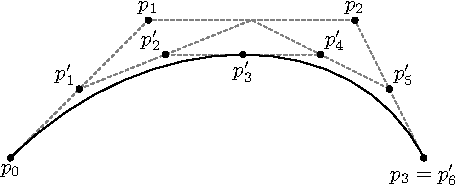
\includegraphics{subdivision}
	     \caption{A Figure}
	 \label{subd}
	\end{figure}

\clearpage %% starts a new page and stops trying to place floats such as tables and figures

\section{More Figure Stuff}
You can also scale and rotate figures.
 	\begin{figure}[h!]
	   
	       \centering
	    % DO NOT ADD A FILENAME EXTENSION TO THE GRAPHIC FILE
	    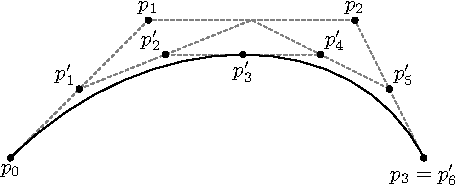
\includegraphics[scale=0.5,angle=180]{subdivision}
	    % if your figure shows up not where you want it, it may just be too big to fit. You can use the scale argument to shrink it, e.g. scale=0.85 is 85 percent of the original size. 
	     \caption{A Smaller Figure, Flipped Upside Down}
	 \label{subd2}
	\end{figure}
	
      \subsection{Common Modifications}
      The following figure features the more popular changes thesis students want to their figures. This information is also on the web at \url{web.reed.edu/cis/help/latex/graphics.html}.
    %\renewcommand{\thefigure}{0.\arabic{figure}} 	% Renumbers the figure to the type 0.x
    %\addtocounter{figure}{4} 						% starts the figure numbering at 4
    \begin{figure}[htbp]
    \begin{center}
   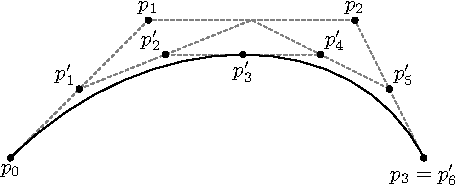
\includegraphics[scale=0.5]{subdivision}
    \caption[Subdivision of arc segments]{\footnotesize{Subdivision of arc segments. You can see that $ p_3 = p_6^\prime$.}} %the special ToC caption is in square brackets. The \footnotesize makes the figure caption smaller
    \label{barplot}
    \end{center}
    \end{figure} 

%If you feel it necessary to include an appendix, it goes here.
    \appendix
      \chapter{The First Appendix}


  \backmatter % backmatter makes the index and bibliography appear properly in the t.o.c...

% if you're using bibtex, the next line forces every entry in the bibtex file to be included
% in your bibliography, regardless of whether or not you've cited it in the thesis.
%    \nocite{*}

% Rename my bibliography to be called "Works Cited" and not "References" or ``Bibliography''
 \renewcommand{\bibname}{Works Cited}

%\bibliographystyle{APA/apa-good}  % or
% \bibliography{thesis}
 % Comment the above two lines and uncomment the next line to use biblatex-chicago.
\printbibliography[heading=bibintoc]

% Finally, an index would go here... but it is also optional.
\end{document}
